
\section{Preservation of the Discrete Maximum Principle}

An important property for a discretization of the TRT equations is preservation of the
discrete maximum principle (MP).  The maximum principle states that the material temperature and mean intensity in the
interior of the domain should be bounded by the solution at the boundaries of the domain, in the
absence of interior energy sources~\cite{wollaber2013discrete,larsen_mpv}.  The analytic solution to the TRT equations satisfies a maximum
principle~\cite{larsen_mpv}, so we desire numerical approximations that preserve the MP in
a discrete sense, for each time step.
%For the discrete MP, we expect the numerical solution to be bounded by the boundary
%conditions at each time step.
For IMC simulations, violation of the maximum principle results in the material
temperature being artificially higher than the radiation temperature.  As discussed in Sec.~\ref{sec:intro}, IMC can violate the MP due to
the approximate linearization of the emission source in the time discretization; it is not
truly implicit in time.  We expect our method, with a fully implicit time discretization,
to preserve the MP with sufficient convergence of the nonlinear emission
source~\cite{larsen_mpv}.

To numerically demonstrate that our method preserves the MP, we have simulated problems
similar to those in~\cite{wollaber2013discrete}.  We modify the Marshak wave problem in
Sec.~\ref{sec:marshak???}, by decreasing $c_v$ and increasing $\sigma_a$, to produce a
problem which results in MP violations for IMC at various fixed time step sizes. 
The spatial and temporal discretization determine the occurence of MP violations for
IMC. In particular, if time steps are too large or spatial
mesh cells are too small, IMC will demonstrate MP violations~\cite{wollaber2013discrete}.  Here, we have kept the
spatial mesh size fixed and increased the time step size to produce MP violations.
The material
specifications for the problem are given in Table~\ref{tab:mpv_prob}. The domain width is 2.0 cm with
$N_c=150$ uniform spatial mesh cells.  The radiation and material energies are initially in
equilibrium at $0.01$ keV, before an isotropic boundary source of $1$ keV is applied at
the left boundary at $t=0$. The simulation end time is $t=0.1$ sh. 

The material and radiation temperature are plotted for an IMC simulation with $\Delta
t=0.025$ sh in
Figure~\ref{fig:imc_mpvrad}.  Figure~\ref{fig:imc_mpv} depicts the material temperature
for various time step sizes and the fixed mesh size of 150 cells. All IMC
simulations used 100,000 histories per time step. As demonstrated in
Fig.~\ref{fig:imc_mpvrad}, the material temperature exceeds the specified boundary
temperature and is artificially hotter than the radiation temperature.  This artificial
``temperature spike'' also leads to a slower propagation of the
wave~\cite{wollaber2013discrete}.  As shown in
Fig.~\ref{fig:imc_mpv}, as larger time-step sizes are taken the nonphysical results worsen.
It is noted that although the final solution for $\Delta t=0.0001$ sh obeys the MP, during
the first few time steps the temperature spikes are present.

The simulations are repeated with the same specifications for the HOLO method. All HOLO
simulations used a fixed mesh of 8 $\mu$ cells by 150 $x$ cells, 3 batches per time step,
and 6,000 histories per batch. A single HO solve is performed per time step, and the LO
relative convergence tolerance is $10^{-6}$. The lumping closure is used in all spatial
cells and any negativities in the HO solution are rotated to the floor value.  

As seen in
Fig.~\ref{fig:holo_mpv}, the HOLO solution does not violate the maximum principle; the
temperature is bounded from above by the radiation boundary condition.
For these simulations, it was
necessary to use the damped Newton's method discussed in Sec.~\ref{sec:damped_newton} to converge the solutions~\cite{damped_newton}. 
 A fixed damping parameter with a factor of 0.5 was found to stably converge for all
 time-step sizes that were simulated. 
Table~\ref{tab:mpv_iters} demonstrates the LO Newton iteration counts for the HOLO method.
For reference, a solution with $\Delta t = 10^{-4}$ sh is given, which required no damping
to converge.  The damped iterations require more iterations to converge.  However, it is necessary to converge the nonlinear iterations to produce
physically meaningful solutions to this problem.  The advantage of the LO solution is that
there is no additional cost for the HO solution when the damped method is used.

\begin{table}[H]
        \caption{\label{tab:mpv_prob}Problem specifications for maximum principle
        violation. Absorption cross section has form $\sigma_a = \sigma_{a,0}/T^3$.}
\centering
        \begin{tabular}{|c|c|} \hline
            $\sigma_{a,0}$ (cm$^{-1}$ keV$^3$)  & 4.0  \\ 
            $\sigma_s$ (cm$^{-1}$) & 0.0 \\
            $\rho$ (g cm$^{-3}$) & 1.0  \\
            $c_v$ (jks/keV-g) & 0.0081181  \\ \hline
        \end{tabular}
\end{table}

\begin{figure}[H]
    \centering
    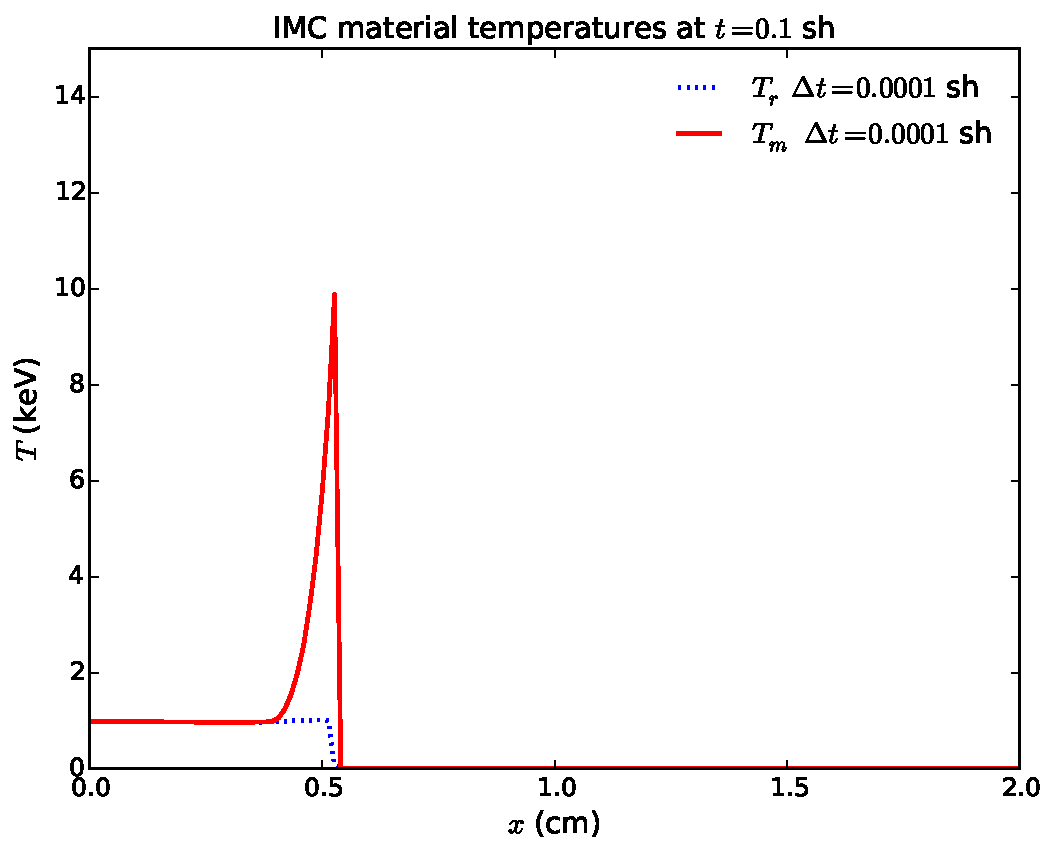
\includegraphics[width=0.6\linewidth]{mpv_rad_imc.pdf}
    \caption{\label{fig:imc_mpvrad}$T_r$ and $T$ for MP violation problem with IMC and $\Delta t = 0.001$ sh.}
\end{figure}

\begin{figure}[H]
    \centering
    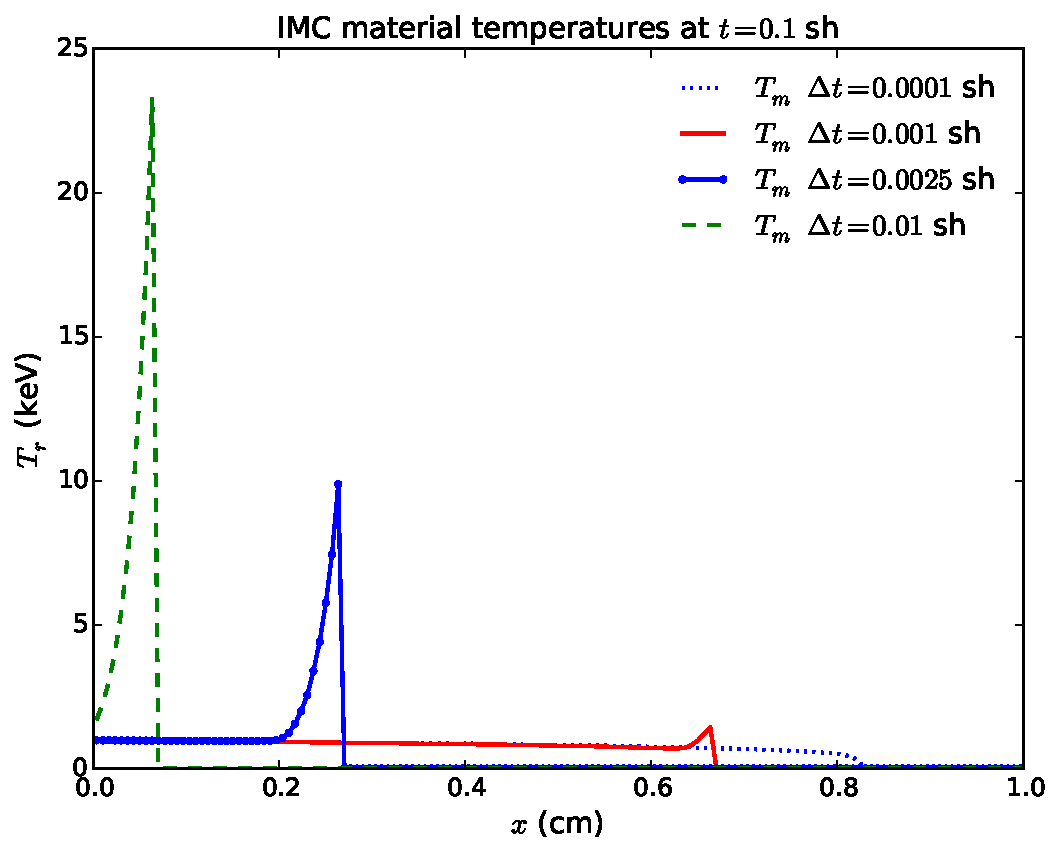
\includegraphics[width=0.6\linewidth]{mpv_mats_imc.pdf}
    \caption{\label{fig:imc_mpv}$T_m$ for MP violation problem with IMC for various time step
    sizes.}
\end{figure}

\begin{figure}[H]
    \centering
    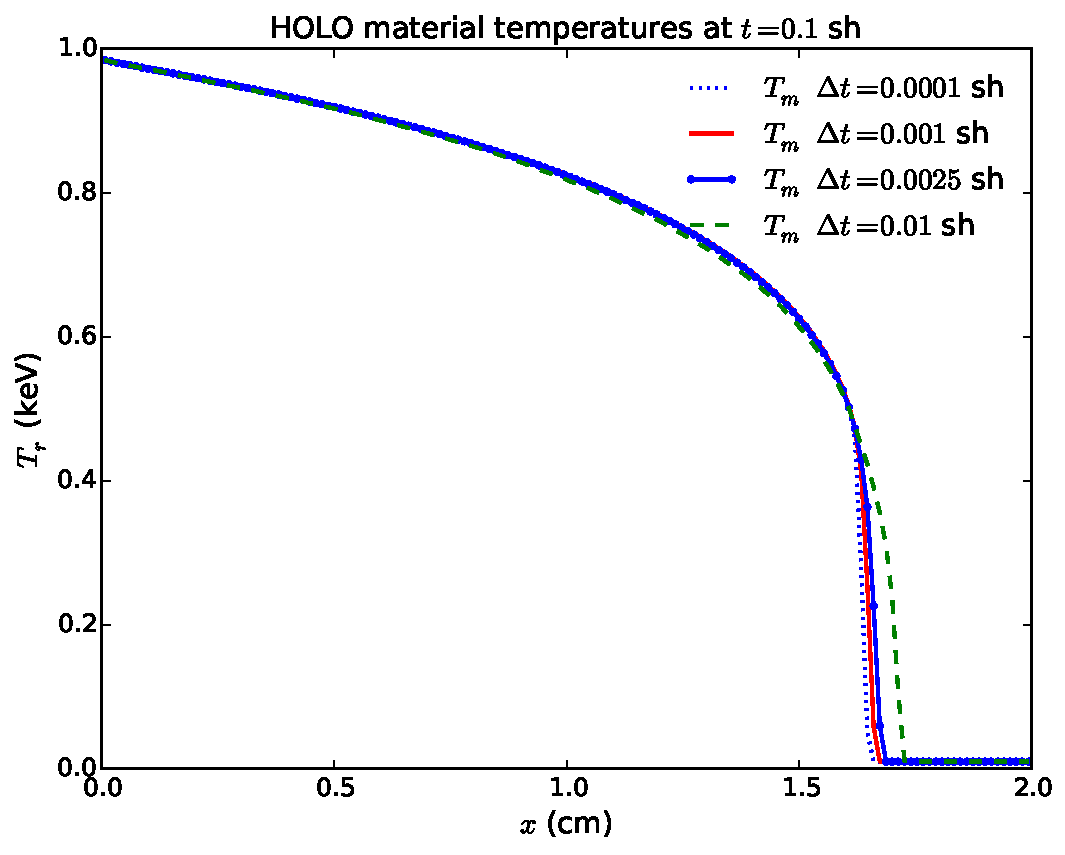
\includegraphics[width=0.6\linewidth]{mpv_mats_holo.pdf}
    \caption{\label{fig:holo_mpv}$T_m$ for MP violation problem with HOLO method for various time step
    sizes.}
\end{figure}

\begin{table}[H]
    \caption{\label{tab:mpv_iters}Comparison of LO Newton iterations for HOLO solution to 
    MP problem and different time step sizes. For $\Delta t=0.1$ sh, no damping was used; for
    all other cases a damping factor of $0.5$ was used.}  
    \centering
        \begin{tabular}{|cc|} \hline
            $\Delta t$ (sh) & Newton Iters. / LO Solve \\ \hline
            $10^{-5}$    & 3.5 \\
            $10^{-4}$    & 21.0 \\
            $10^{-3}$    & 28.5 \\
            $2.5\times10^{-3}$  & 29.7 \\
            $10^{-2}$    & 46.3 \\ \hline
        \end{tabular}
\end{table}

